\documentclass[11pt]{beamer}
\usepackage[utf8]{inputenc}
%\usepackage[]{babel}
\usepackage{amsmath}
\usepackage{amsfonts}
\usepackage{amssymb}
\usepackage{graphicx}
\usetheme{Boadilla}

\makeatother
\setbeamertemplate{footline}
{
	\leavevmode%
	\hbox{%
		\begin{beamercolorbox}[wd=.33\paperwidth,ht=2.25ex,dp=1ex,center]{author in head/foot}%
			\usebeamerfont{author in head/foot}\insertshortauthor
		\end{beamercolorbox}%
		\begin{beamercolorbox}[wd=.34\paperwidth,ht=2.25ex,dp=1ex,center]{title in head/foot}%
			\usebeamerfont{title in head/foot}\insertshorttitle
		\end{beamercolorbox}%
		\begin{beamercolorbox}[wd=.33\paperwidth,ht=2.25ex,dp=1ex,center]{date in head/foot}%
			\usebeamerfont{date in head/foot}\insertshortdate{}\hspace*{2em}\insertframenumber{} / \inserttotalframenumber
	\end{beamercolorbox}}%
	\vskip0pt%
}

% Package to insert code
\usepackage{xcolor}
\usepackage{listings}
\lstset{language=[ISO]C++}					%set code language
\lstset{basicstyle=\small\ttfamily,
	keywordstyle = \color{blue}\bfseries,
	commentstyle = \color{gray},
	stringstyle = \color{green},
	morecomment=[l][\color{magenta}]{\#}}	% code style
\lstset{tabsize=2}							% tabulation for code
\lstset{backgroundcolor = \color{yellow!7}}	% sfondo
%\lstset{numbers=left, numberstyle=\tiny}	% numerazione righe
\lstset{aboveskip=10pt, belowskip=10pt}		% spaziatura prima e dopo il codice
\newcommand{\classname}[1]{\texttt{#1}}

\AtBeginSection[]{
	\begin{frame}
		\vfill
		\centering
		\begin{beamercolorbox}[sep=8pt,center,shadow=true,rounded=true]{title}
			\usebeamerfont{title}\insertsectionhead\par%
		\end{beamercolorbox}
		\vfill
	\end{frame}
}

\author{Speranza Ilaria \\ Tantardini Mattia}
\title{BGLgeom Library}
%\subtitle{}
%\logo{}
\institute{\textbf{Politecnico di Milano}}
\date{March 2, 2017}
\subject{Advanced Programming for Scientific Computing}
%\setbeamercovered{transparent}
%\setbeamertemplate{navigation symbols}{}

\begin{document}
	\begin{frame}
		\maketitle
	\end{frame}
	
	\begin{frame}
		\frametitle{Project's objectives}
		\begin{itemize}
			\item Add geometric features to a BGL graph 
			\item Implement linear, b-spline and "generic" edges
			\item Provide mesh generator on each edge
			\item Handle I/O operations from/to useful formats (.pts, .vtp, ASCII) 
			\item Fracture\_intersection and Network\_diffusion applications 
		\end{itemize}
	\end{frame}
	
	\section{The library}
	\begin{frame}
		\frametitle{Briefs on Boost Graph Library}
		\begin{block}{Adjacency\_list}
			\texttt{adjacency\_list< OutEdgeList, VertexList, Directed, VertexProperties, EdgeProperties >} \newline
			Template class representing the graph with a two dimensional structure: 
			a \texttt{VertexList}, containing all the vertices, and an \texttt{OutEdgeList} associated to each vertex, containing all its out-edges.
		\end{block}
		
		\begin{block}{Vertex \& Edge descriptors and iterators}
			Descriptors are the types for vertices and edges representative objects; iterators allow to traverse graph's vertex and edge sets.
		\end{block}
		
		\begin{block}{Bundled properties}
			Structs associated to each vertex and each edge containing their properties and methods
		\end{block}	
	\end{frame}
	
	\begin{frame}
		\frametitle{BGLgeom}
		This library has been developed to provide an environment where building and running all those applications which have both a graph topological structure and a geometric description for vertices (position in the space) and edges (which could not be linear).\\
		BGLgeom implements also some input/output utilities, to make this library 'compatible' with other softwares.
	\end{frame}
	
	\begin{frame}{Inside BGLgeom}
		\begin{itemize}
			\item \textbf{Adapters for BGL}: layers and additional functions to hidden the most used native BGL ones and to improve readibility and ease of use.
			\item \textbf{Classes to build graph properties}: the main part of the library; classes to be associated vertices and edges
			as properties including the basic geometric requirements.
			\item \textbf{Geometrical and numerical utilities}: Code to compute integrals, generate meshes, compute intersections between linear edges.
			\item \textbf{I/O utilities}: one reader class to read tabular ASCII files, and three writer classes to produce three different types of output: ASCII, .pts and .vtp files.
			\item \textbf{Tests}: source code examples to show how the main classes and writers work.
		\end{itemize}
	\end{frame}
	
	\begin{frame}
		\frametitle{Geometric properties}
		We implemented the geometrical properties we were required as \textit{bundled properties}, which are then associated to each single vertex and edge.
		\begin{block}{Vertex\_base\_property}
			\begin{itemize}
				\item coordinates, describing the physical location of the point in the space
				\item boundary conditions (possibly more than one)
				\item label
				\item index
			\end{itemize}
		\end{block}
		\begin{block}{Edge\_base\_property}
			\begin{itemize}
				\item geometry (linear, b-spline, generic)
				\item mesh
				\item label
				\item index
			\end{itemize}
		\end{block}		
	\end{frame}
	\begin{frame}
		\frametitle{Edge geometry abstract class}
		All geometry classes derive from an abstract class, \texttt{edge\_geometry}, which specifies the functionalities that the geometry of an edge should have: evaluation of the curve, computation of first and second derivative, curvature and curvilinear abscissa at given value (or a vector of values) of the parameter. All the classes hold a parameterization of the curve between 0 and 1, so we actually have parameterizations of the type
		\begin{equation*}
		f:[0,1]\rightarrow\mathbb{R}^{n} \quad, \quad n=2,3.
		\end{equation*}
		for each geometry.
	\end{frame}
	\begin{frame}
		\frametitle{Concrete edge geometries}
		\begin{itemize}
			\item \textbf{Linear geometry} describes straight lines. It stores as internal attributes the coordinates of the source and the target of the edge. The coordinates of source and target are used to rescale the parameterization from [0,1] to the real position in the space. 
			\item \textbf{Generic geometry} can store the exact parameterization of any curve; it requires to provide the exact analytic expression of the curve and of its first and second derivative, each one parametrized between 0 and 1.
			\item \textbf{Bspline geometry} stores as private attributes the control points and the knot vectors for the curve and for its first and second derivatives.	
			The user can choose between interpolating and approximating b-splines.
		\end{itemize}
	\end{frame}

	\defverbatim[colored]\lstI{
	\begin{lstlisting}[language=C++,basicstyle=\small\ttfamily,keywordstyle=\color{red}]
	#include <boost/graph/adjacency_list.hpp>
	#include "base_properties.hpp"
	
	using Edge_prop = 
		BGLgeom::Edge_base_property
			<BGLgeom::linear_geometry<3>,3>;
	using Vertex_prop = BGLgeom::Vertex_base_property<3>;
	using Graph = 
		boost::adjacency_list<boost::vecS, boost::vecS,
			boost::directedS, Vertex_prop, Edge_prop>;
	
	Graph G;
	\end{lstlisting}
	}
	
	\begin{frame}
		\frametitle{Example: declaring a geometric graph}
		\lstI
	\end{frame}
		
	\defverbatim[colored]\lstII{
	\begin{lstlisting}[language=C++,basicstyle=\small\ttfamily,keywordstyle=\color{red}]
	#include "base_properties.hpp"
	
	struct My_edge_prop : 
		public BGLgeom::Edge_base_property<3> {
			double variable1;			// may be pressure
			int varaible2;				// some flag
			std::string a_string;	// a description
			my_class object;			
	
			My_edge_prop() : 
				BGLgeom::Edge_base_property<3>(),
				variable1(.0),
				variable2(0),
				a_string(),
				object() {};	
	};
	\end{lstlisting}
	}
	
	\begin{frame}
		\frametitle{Example: extending base properties}
		\lstII|
	\end{frame}

	\defverbatim[colored]\lstIII{
	\begin{lstlisting}[language=C++,basicstyle=\small\ttfamily,keywordstyle=\color{red}]
	#include "graph_access.hpp"
	#include "graph_builder.hpp"
	#include "base_properties.hpp"		
	#include "point.hpp"
	
	using Edge_prop = 
		BGLgeom::Edge_base_property
			< BGLgeom::linear_geometry<3>, 3 >;
	using Vertex_prop = BGLgeom::Vertex_base_property<3>;
	using Graph = 
		boost::adjacency_list< boost::vecS, boost::vecS, 
			boost::directedS, Vertex_prop, Edge_prop >;
	\end{lstlisting}
	}

	\defverbatim[colored]\lstIIII{
	\begin{lstlisting}[language=C++,basicstyle=\small\ttfamily,keywordstyle=\color{red}]
	Graph G;
	BGLgeom::Vertex_desc<Graph> src, tgt;
	BGLgeom::Edge_desc<Graph> e;
	
	src = BGLgeom::new_vertex(G); // add a new vertex 
	tgt = BGLgeom::new_vertex(G); // add another vertex
	
	// set src coordinates
	G[src].coordinates = BGLgeom::point<3>(1,1,1); 
	// set tgt coordinates
	G[tgt].coordinates = BGLgeom::point<3>(2,2,2); 
	
	// add an edge connecting src to tgt
	e = BGLgeom::new_linear_edge(src, tgt, G);
	// set edge's index	
	G[e].index = 1;
	\end{lstlisting}
	}
	
	\begin{frame}
	\frametitle{Example: Adding vertices and edges}
	\lstIII|
	\end{frame}

	\begin{frame}
	\lstIIII
	\end{frame}
	
	\begin{frame}
		\frametitle{Reader class}
		We provided in this library a generic ASCII reader to read topology and properties of the graph from a tabular file. The reader is a template abstract class; while deriving his own concrete reader, the user has to specify:
		\begin{itemize}
			\item all the attributes to be stored while reading;
			\item \texttt{get\_data()}: how to read (in the right order) from the file the data for each single edge, using the inner stream attribute;
			\item \texttt{get\_source\_data()} and \texttt{get\_target\_data()}: how to pack the data into the vertex property of source and target of the edge currently read;
			\item \texttt{get\_edge\_data()}: how to pack the data into the edge property which will be assigned to the new edge ;
			\item \texttt{get\_topological\_data()}: if topological information are provided, how to "exploit" them, otherwise an empty struct (the default \texttt{BGLgeom::no\_topological\_data} is provided in the same header).
		\end{itemize}
	\end{frame}
	
	\begin{frame}
		\frametitle{Writer classes}
		Three kinds of writers are provided to output the graph and its properties; each one produces a different format of output.
		\begin{itemize}
			\item{Writer\_ASCII} produces as output a tabular format (.txt, .dat, etc). It is an abstract class with the same philosophy as the \texttt{reader\_ASCII} class: the user has to define its concrete writer, specifying which properties of the graph to print, and how.
			\item{Writer\_pts} produces the output in a particular format (.pts): it expresses the graph as a sequence of arcs, and for each arc the boundary conditions on source and target and all points of the mesh defined on it (if present) are printed. 
			\item{Writer\_vtp} produces a .vtp output, i.e. a VTK polygonal data format. The output consists into two files: one coding the edges, and one coding the vertices of the graph. This kind of output is thought to visualization purpouse: using for instance software such as Paraview, the output files can be easily displayed.
		\end{itemize}
		\end{frame}			
		
		\begin{frame}
			\frametitle{Future developments}
			\begin{block}{Dynamic edge properties}
				The \classname{Edge\_base\_property} is passed as template parameter to create the graph, which implies that the geometry of all the edges in the graph is be fixed. This behaviour may be inefficient for some applications, for instance when the underlying graph has almost all linear edges and only few edges with complex geometry.It may be interesting to implement a 'dynamic' version of the \classname{Edge\_base\_property}, which allows the user select a different geometry on each edge in the graph.
			\end{block}
			\begin{block}{B-spline interpolation}
				At present, the interpolation method for b-splines works only with uniform knots and in the cubic case. It may be useful to implement more general methods.
			\end{block}
		\end{frame}
	
	\section{Applications}
	\begin{frame}
		\frametitle{Fracture intersection}
			A list of fractures, all lying on the same plane, is given as input. \\
			The goal is to build a graph representing the network, with vertices in correspondence of the fractures' extremities and of the intersection points and edges representing the fractures.
	\end{frame}

	\defverbatim[colored]\lstfrac{
	\begin{lstlisting}[language=C++,basicstyle=\small\ttfamily,keywordstyle=\color{red}]
	while(!eof){
		fracture = getline()
		create fracture edge_property 
		int_vect.clear()
		for e in edges(G){
			compute_intersection(e, fracture)
			if intersection exists{
				create Int_Layer with intersection information
				int_vect.push_back(Int_Layer)
			}	
		}
		if int_vect.empty(){
			add_edge to graph with fracture edge properties
		} else {
			reorder int_vect
			remove_duplicates inside int_vect
			refine_graph(fracture, int_vect)  
		}
	}
	\end{lstlisting}
	}

	\begin{frame}{The algorithm}
		\lstfrac
	\end{frame}

	\begin{frame}{Intersection types}
		\begin{figure}
		\centering 
		\includegraphics[width=1\textwidth]{"int_type"}
		\end{figure}
	\end{frame}

	\begin{frame}{Example on duplicates removal}
		\begin{figure}
			\centering 
			\includegraphics[width=1\textwidth]{"rem_dupl"}
		\end{figure}
	\end{frame}

	\begin{frame}{Graph building step by step}
		\begin{figure}
			\centering 
			\includegraphics[width=.9\textwidth]{"graph_building_process"}
		\end{figure}
	\end{frame}

	\begin{frame}{Handling 'real' data}
		\begin{figure}
			\centering 
			\includegraphics[width=.9\textwidth]{"graph1"}
			\caption{fractureElevenVF.dat}
		\end{figure}
	\end{frame}

	\begin{frame}
		\begin{figure}
			\centering 
			\includegraphics[width=.9\textwidth]{"graph2"}
			\caption{fractures.txt}
		\end{figure}
	\end{frame}

		\begin{frame}
		\frametitle{Coupled problem on one dimensional network}
		\framesubtitle{Application to microcirculation}
		The goal is to solve a fluid transport problem ina permeable biological tissue perfused by a capillary network. The whole domain $\Omega$ is divided into the tissue volume $\Omega_{t}$ and the capillary bed $\Omega_{v}$. The latter is reduced from a 3D to a 1D description, thus generating a graph for the capillary network, where the edges are straight lines.
		\newline\newline
		The quantity of interest is the concentration of transported solute $c$, function of space and time. The wall of capillaries is assumed permeable, so that solute can flow from vessels to tissue.
		\newline\newline
		Boundary conditions are imposed on the capillary network so that the mass goes from $\Gamma_{\textit{inflow}}$ to $\Gamma_{\textit{outflow}}$, being them the external communicating sections of the vessels.
	\end{frame}
	
	\begin{frame}
		\frametitle{Our role}
		The problem was substantially already solved thanks to code developed in previous and ongoing PACS project and based on GetFEM++ solvers. The remaining issue was a comprehensive description and generation of the underlying graph for the capillary network. Here we gave our contribution:
		\begin{itemize}
			\item We first of all developed a Matlab script to generate a random capillary networks with successive bifurcations in orthogonal planes; it produces a file with the coordinates of source and target of the edges in each row.
			\item Then we used our BGLgeom library to read the input file with the generated capillary network and build the corresponding graph, setting properly coordinates and BCs on the vertices.
			\item We generated a uniform mesh on each edge.
			\item Finally we output the graph in .pts format, ready to be read by the GetFEM++ solver.
		\end{itemize}	
	\end{frame}
	
	\begin{frame}
		\frametitle{The capillary network}
		\begin{figure}
			\centering
			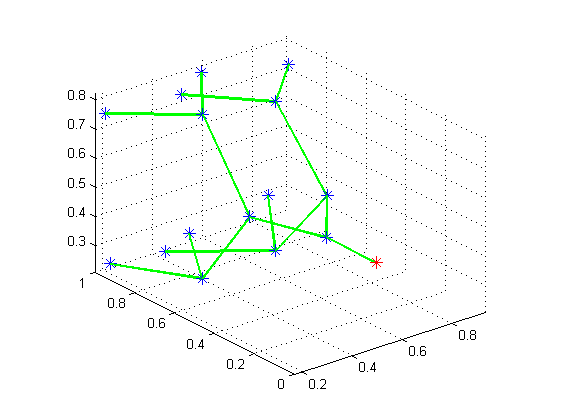
\includegraphics[width=.65\textwidth]{capillary_network}
		\end{figure}
		The network was generated with 4 orders of bifurcations and random coefficient 0.05. The red dot is the inflow border, while all the extremities on the other side are outflow borders.
	\end{frame}
	
	\begin{frame}
		\frametitle{The results}
		On that capillary network we solved a stationary diffusion problem. The results correctly show that the mass diffuses into the network and then flows through the vessel walls into the surrounding tissue.
		\begin{figure}[h]
			\centering
			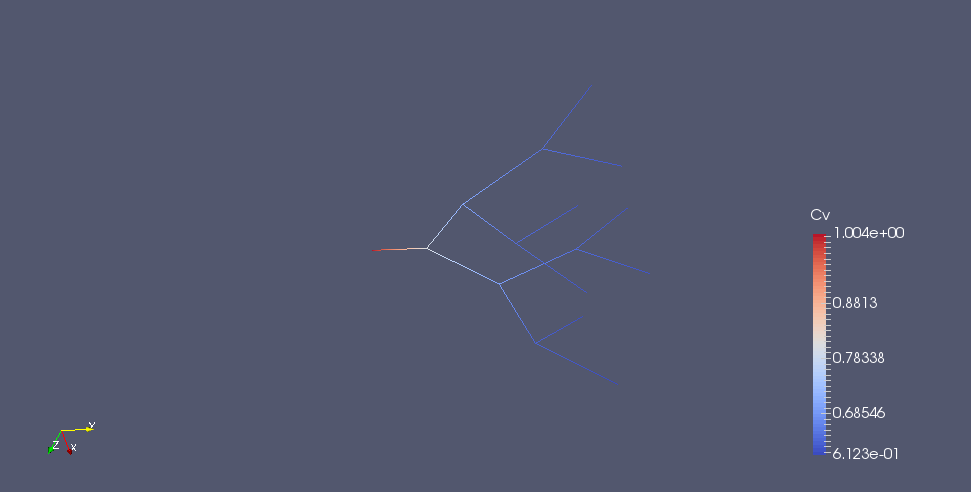
\includegraphics[width=0.8\linewidth]{cv}
			\label{fig:cv}
		\end{figure}
	\end{frame}
	
	\begin{frame}
		\frametitle{The results (2)}
		\begin{figure}[!h]
			\centering
			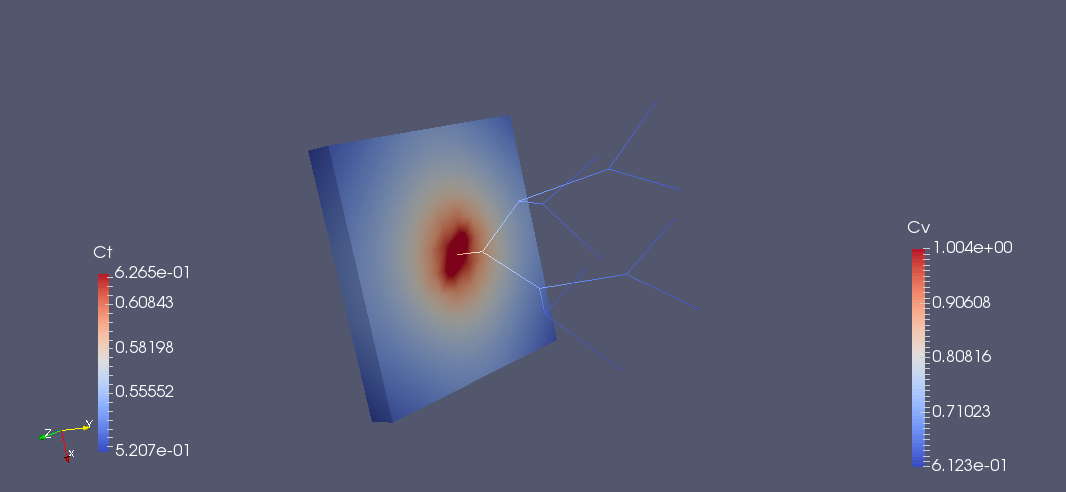
\includegraphics[width=0.9\linewidth]{ct1}
			\label{fig:ct1}
		\end{figure}
	\end{frame}
	
	\begin{frame}
		\frametitle{The results (3)}
		\begin{figure}[!h]
			\centering
			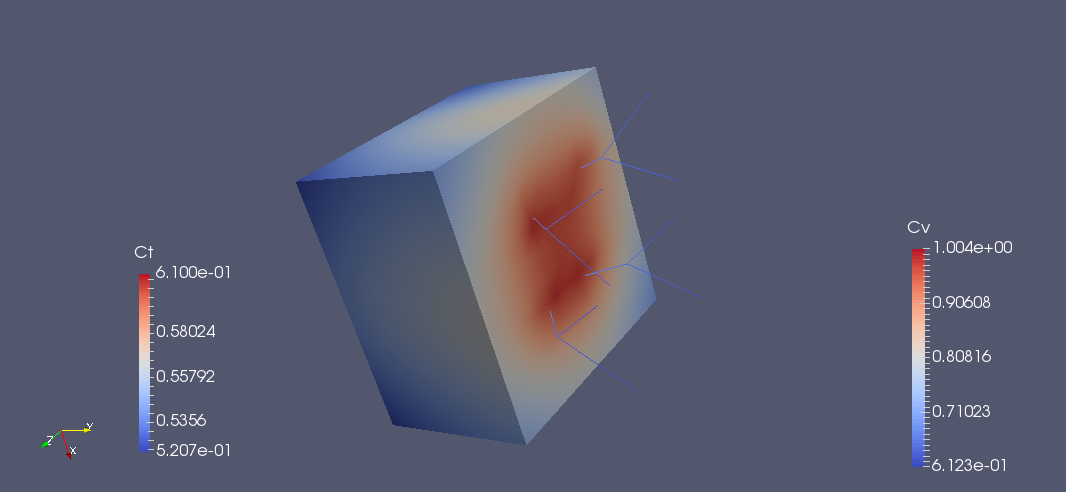
\includegraphics[width=0.9\linewidth]{ct2}
			\label{fig:ct2}
		\end{figure}
	\end{frame}
	
	\begin{frame}
		\frametitle{The results (4)}	
		\begin{figure}[!h]
			\centering
			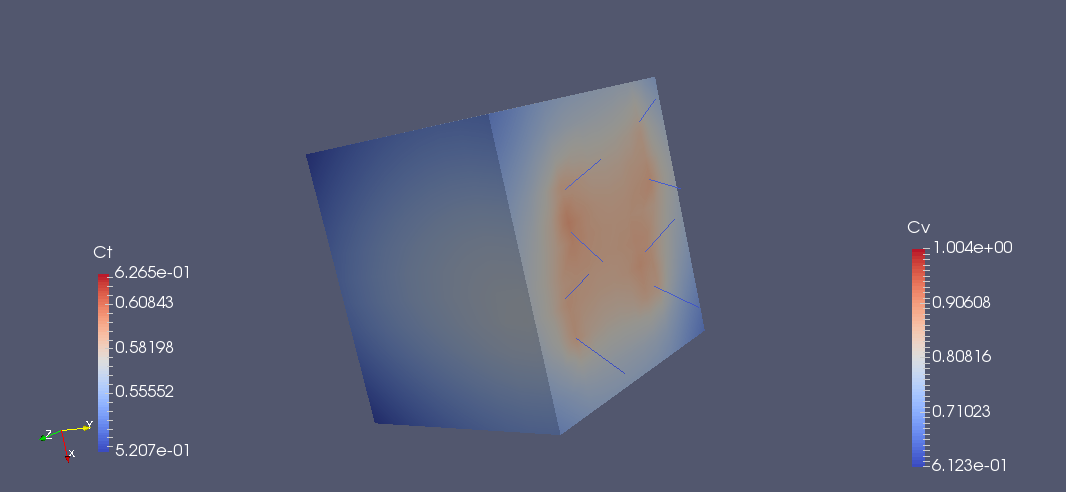
\includegraphics[width=0.9\linewidth]{ct3}
			\label{fig:ct3}
		\end{figure}
	\end{frame}

	\begin{frame}{References}
		\begin{itemize}
			\item Jeremy Siek/Lie-Quan Lee/Andrew Lumsdaine, \textit{The Boost Graph Library - User guide and reference manual}, Addison-Wesley, 2002.
			\item Tomas Sauer, \textit{Splines in Industrial Applications}, 2007, concerning b-spline interpolation.
			\item \textit{http://www.boost.org/doc/libs/1\_61\_0/libs/graph/doc/}, BGL website.
			\item \textit{http://www.gnu.org/software/make/manual/make.html}, for some support on Makefile.
			\item \textit{http://eigen.tuxfamily.org/dox}, Eigen documentation.
			\item \textit{http://www.stack.nl/~dimitri/doxygen/manual/index.html}, Doxygen documentation.
			\item \textit{http://www.vtk.org/Wiki/VTK/Examples}, some documentation and examples on usage of VTK library.
			\item \textit{www.stackoverflow.com}.
		\end{itemize}
	\end{frame}

\end{document}
